\section{Introduction}\label{sec:intro}

The \gls{hms} is a \acrlong{swe} model and solver, developed in-house at the Chair of Water Resources Management and Modeling of Hydrosystems.
The \glspl{swe} are used to model shallow water flow, e.g., flooding in cases of heavy rainfall events, the behavior of river systems, and urban interventions like green roofs \autocite{fischer2024,sanders2008}.

A core motivation for developing \gls{hms} has been enabling the use of \acrlong*{2D} \gls{swe} models in large-scale high-resolution systems by shifting their applicability limit.
The lower limit consists of considerations whether a model can represent a certain detail relevant for a specific task, and can be thought of as a \emph{hard limit}.
In contrast, the upper limit can be regarded simply as the cost and practicability of running a simulation and therefore represents a \emph{soft limit} \autocite{lennart-hms}.

\begin{figure}[htbp]
	\centering
	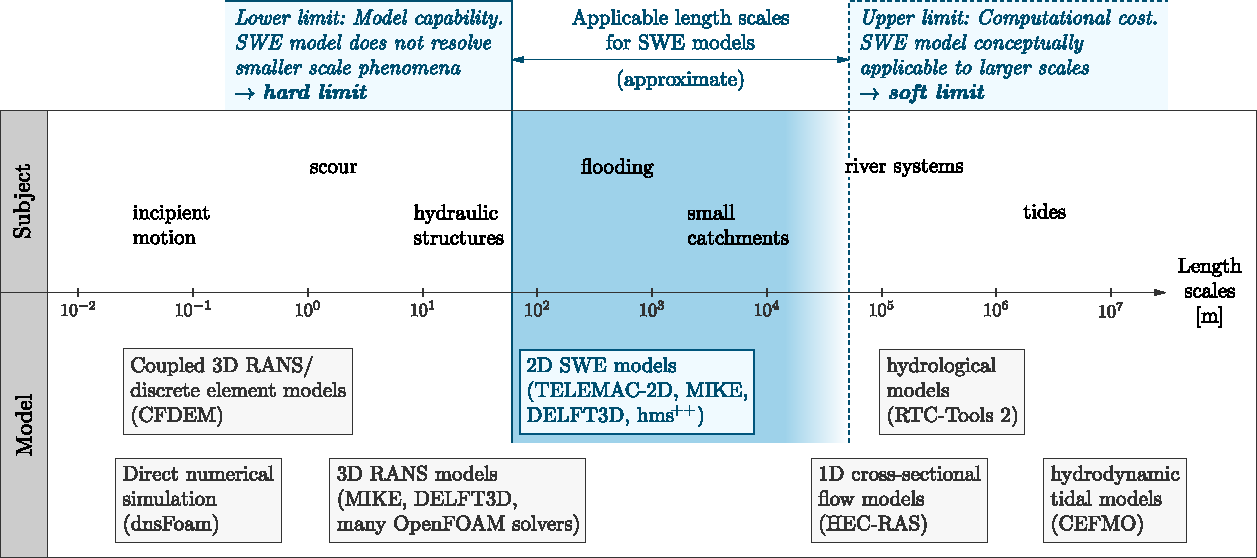
\includegraphics[width=\textwidth]{./img/length_scales_rev.pdf}
	\caption
    [Subjects of interest in fluid flow at their characteristic length scales]
    {
		``Subjects of interest in fluid flow at their characteristic length scales, and models (with software examples in brackets) at their applicable length scales (approximate).''
		\autocite{lennart-hms}
	}
\end{figure}

Because of this, improving computational performance has always been a central goal in the development of \gls{hms}.
Therefore, parallel processing methods and other optimization techniques have been included in its conceptualization from the very beginning \autocite{steffen2020}.

A method for increasing performance that is currently not implemented, is \acrlong*{lts}: the idea of locally reducing computations where it is possible while still maintaining stability and accuracy. 
To accurately solve the \glspl{swe} in practical cases, numerical methods are required:
the domain is spatially discretized into cells; the simulation duration is explicitly discretized into periods of dynamic length, i.e., time steps.
A stability criterion limits these time step lengths according to cell size, maximum propagation velocity, and the Courant number.
The \acrlong*{gts} scheme, which is currently used in \gls{hms}, limits the global time step to the minimum value obtained by applying the stability criterion on each cell in the domain. The stability criterion is thus applied globally.
\Acrlong*{lts} schemes use different time steps throughout the domain by applying the stability criterion locally to reduce the number of computations.
As these computations are complex and therefore costly, the runtime of a \gls{swe} solver decreases with the number of computations.
On the other hand, the use of a \acrlong*{lts} bears the risk of introducing instabilities and hurting accuracy.

The implementation of a \acrlong*{lts} scheme in \gls{hms} is required to build upon optimization techniques currently in use.
Primarily, the block-wise traversal is obliged to be maintained, as it has proven to benefit performance immensely by enabling effective parallelization and cache utilization \autocite{lennart-conf}.

Thus, a novel \acrlong*{lts} method is developed and implemented within \gls{hms}.
\autoref{sec:background} outlines background resources required for this task, including governing equations, discretization, and existing \acrlong*{lts} schemes.
\autoref{sec:methods} describes specifics of the proposed time stepping scheme, implementation details, as well as test cases. 
These consist of an analytically solvable \acrlong{1D} dam break case and an example of urban rainfall-runoff.
\autoref{sec:results} covers accuracy and runtime analysis of these test cases.
Finally, \autoref{sec:conclusion-outlook} presents a conclusive summary, as well as an outlook into possible future research. 
